\documentclass[sn-nature]{sn-jnl}

\usepackage{graphicx}
\usepackage{multirow}
\usepackage{amsmath,amssymb,amsfonts}
\usepackage{booktabs}
\usepackage{tabularx}
\usepackage{xcolor}
\usepackage{tikz}
\usetikzlibrary{positioning,calc,arrows.meta,fit}

\newcommand \RR {\mathbb{R}}
\DeclareMathOperator*{\diag}{Diag}

\newcommand{\CRANpkg}[1]{\href{https://CRAN.R-project.org/package=#1}{\textbf{#1}}}
\newcommand{\code}[1]{\texttt{#1}}

\raggedbottom

\definecolor{HeaderBlue}{HTML}{183B56}
\definecolor{RowBlue}{HTML}{F2F7FB}
\definecolor{YesBackground}{HTML}{DDF2E3}

\begin{document}
\title[Benchmarking sparse GRN inference on gastruloids]{Comparative analysis of sparse gene-regulatory network inference on murine gastruloid single-cell RNA-seq}

\author*[1,2]{\fnm{Bastien} \sur{Chassagnol}}
\email{bastien\_chassagnol@laposte.net}
\equalcont{B.C.\ and M.P.\ contributed equally to this work.}

\author[3]{\fnm{Marielle} \sur{P\'{e}r\'{e}}}
\email{marielle.pere@inria.fr}
\equalcont{B.C.\ and M.P.\ contributed equally to this work.}

\author[1]{\fnm{Mohamad} \sur{Al Charif}}

\author[2]{\fnm{Gr\'{e}gory} \sur{Nuel}}
\email{nuel@math.cnrs.fr}

\author[4]{\fnm{Etienne} \sur{Becht}}
\email{etienne.becht@inserm.fr}

\author[1]{\fnm{Ana\"{i}s} \sur{Baudot}}
\email{anais.baudot@univ-amu.fr}

\affil[1]{\orgdiv{Marseille Medical Genetics (MMG), Systems Biomedicine team},
  \orgname{Aix-Marseille University, Inserm U1251},
  \orgaddress{\street{Facult\'{e} de M\'{e}decine, 27 Bd Jean Moulin},
    \city{Marseille}, \postcode{13385}, \country{France}}}

\affil[2]{\orgdiv{Laboratoire de Probabilit\'{e}s, Statistique et
  Mod\'{e}lisation (LPSM), UMR 8001},
  \orgname{Sorbonne Universit\'{e} / CNRS},
  \orgaddress{\city{Paris}, \country{France}}}

\affil[3]{\orgdiv{MacBes team},
  \orgname{Inria Centre at Universit\'{e} C\^{o}te d'Azur;
    Institut de Pharmacologie Mol\'{e}culaire et Cellulaire (IPMC)},
  \orgaddress{\city{Sophia-Antipolis}, \country{France}}}

\affil[4]{\orgdiv{Centre de Recherche sur l'Inflammation (CRI),
  UMR 1149},
  \orgname{Inserm / Universit\'{e} Paris Cit\'{e}},
  \orgaddress{\street{Facult\'{e} de m\'{e}decine -- site Bichat,
    16 rue Henri Huchard},
    \city{Paris}, \postcode{75018}, \country{France}}}

\abstract{Organoid and gastruloid models reduce the need for in vivo
experiments, but interpreting their transcriptomes requires maps of
gene--gene dependence. We outline a benchmark of gene-regulatory
network (GRN) inference on gastruloid single-cell RNA-seq, restricted
here to two sparse Gaussian graphical model (GGM) estimators---the
frequentist package SILGGM and the Bayesian latent mixture BLGGM---and
an optional directed tree ensemble (GRNBoost2) as a topological
comparator. Networks are compared by engineering cost, runtime and
edge-set overlap (raw and chance-adjusted Jaccard), not by a gold
standard. The companion code lives in the DeCovarT reproducibility
repository.}

\keywords{gene regulatory network, Gaussian graphical model, scRNA-seq, gastruloid}

\maketitle

\section{Introduction}
\label{sec1}

To study genetic disease while reducing in vivo work, biologists grow
three-dimensional structures that mimic organ development (organoids).
Gastruloids are organoids that recapitulate gastrulation-stage
patterning. Understanding how genes jointly build tissue requires GRN
inference: a weighted graph or an adjacency table
(Fig.~\ref{fig:grn_table}).

This manuscript recasts an M1 internship benchmark
on gastruloid scRNA-seq from Suppinger and colleagues
\cite{suppingerMultimodalCharacterizationMurine2023}. We drop graph-neural
methods that inject literature embeddings and keep two precision-matrix
estimators: SILGGM \cite{zhangSILGGMExtensivePackage2018} and BLGGM
\cite{wuEstimatingHeterogeneousGene2022}, both descendants of the
graphical lasso \cite{friedmanSparseInverseCovariance2008}.
GRNBoost2 remains a directed, dense tree-ensemble comparator
\cite{moermanGRNBoost2ArboretoEfficient2019}, as used in SCENIC
\cite{aibarScenicSinglecellRegulatory2017}.

\section{Methods}
\label{sec2}

\subsection{Data}
We use gastruloid scRNA-seq \cite{suppingerMultimodalCharacterizationMurine2023}.
Rows are cells and columns are genes. The original object has 2{,}819
cells and about 27{,}000 genes. We retain the 500 genes of largest
marginal variance as a computational filter, not as a leakage-free
signature for deconvolution.

\subsection{Hardware}
Experiments were run on the laboratory cluster: Ubuntu 22.04.5 LTS, 40
CPU cores, NVIDIA RTX 5000 Ada (32\,GB), CUDA 12.2. Reproducible R
jobs in this repository use at most two cores on CI.

\subsection{Estimators}
All methods take the same filtered expression table (plus optional
transcription-factor lists for GRNBoost2).

\paragraph{GRNBoost2.}
Gradient-boosted trees per target gene in the Arboreto framework
\cite{moermanGRNBoost2ArboretoEfficient2019}, the scalable engine used
by SCENIC \cite{aibarScenicSinglecellRegulatory2017}. Input: expression
matrix and a transcription-factor dictionary. Output: a directed,
typically dense network.

\paragraph{BLGGM.}
Bayesian latent Gaussian graph mixture
\cite{wuEstimatingHeterogeneousGene2022}. Latent Gaussians per cell
type, non-ignorable dropout, spike-and-slab precision matrices. Output:
sparse undirected graphs after MCMC.

\paragraph{SILGGM.}
Frequentist high-dimensional GGM inference with FDR control
\cite{zhangSILGGMExtensivePackage2018}. After a nonparanormal
transform \cite{liuNonparanormalSemiparametricEstimation2009} implemented
in \CRANpkg{huge} \cite{R-huge}, de-sparsified graphical lasso or related
tests yield a sparse undirected graph.

\subsection{Benchmark pipeline}
GRN inference is unsupervised: there is no tissue-wide gold standard.
We therefore compare consensus among methods (Fig.~\ref{fig:pipeline}).
Directed edges from GRNBoost2 are symmetrised before Jaccard
comparison with undirected GGMs.

\begin{figure}[t]
  \centering
  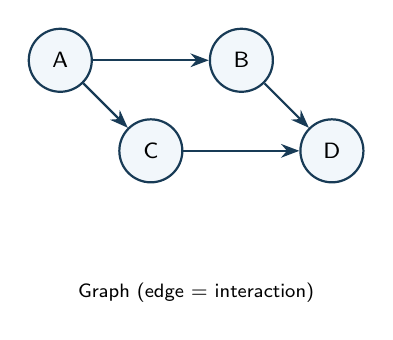
\begin{tikzpicture}[x=1.15cm, y=1.15cm, font=\sffamily\footnotesize]
    \foreach \name/\x/\y in {A/0/2, B/2/2, C/1/1, D/3/1} {
      \node[circle, draw=HeaderBlue, thick, fill=RowBlue,
        minimum size=8mm] (\name) at (\x,\y) {\name};
    }
    \draw[HeaderBlue, thick, -{Stealth}] (A) -- (B);
    \draw[HeaderBlue, thick, -{Stealth}] (A) -- (C);
    \draw[HeaderBlue, thick, -{Stealth}] (B) -- (D);
    \draw[HeaderBlue, thick, -{Stealth}] (C) -- (D);
    \node[font=\sffamily\scriptsize, anchor=north] at (1.5,-0.35)
      {Graph (edge $=$ interaction)};
  \end{tikzpicture}
  \hfill
  \begin{tabular}{lcccc}
    \toprule
    & A & B & C & D \\
    \midrule
    A & 0 & 1 & 1 & 0 \\
    B & 1 & 0 & 0 & 1 \\
    C & 1 & 0 & 0 & 1 \\
    D & 0 & 1 & 1 & 0 \\
    \bottomrule
  \end{tabular}
  \caption{A GRN as an undirected graph (left) and a binary adjacency
    table (right). Entry $1$ marks an edge; $0$ marks none. Layout
    follows the internship schematic without raster artwork.}
  \label{fig:grn_table}
\end{figure}

\begin{figure*}[t]
  \centering
  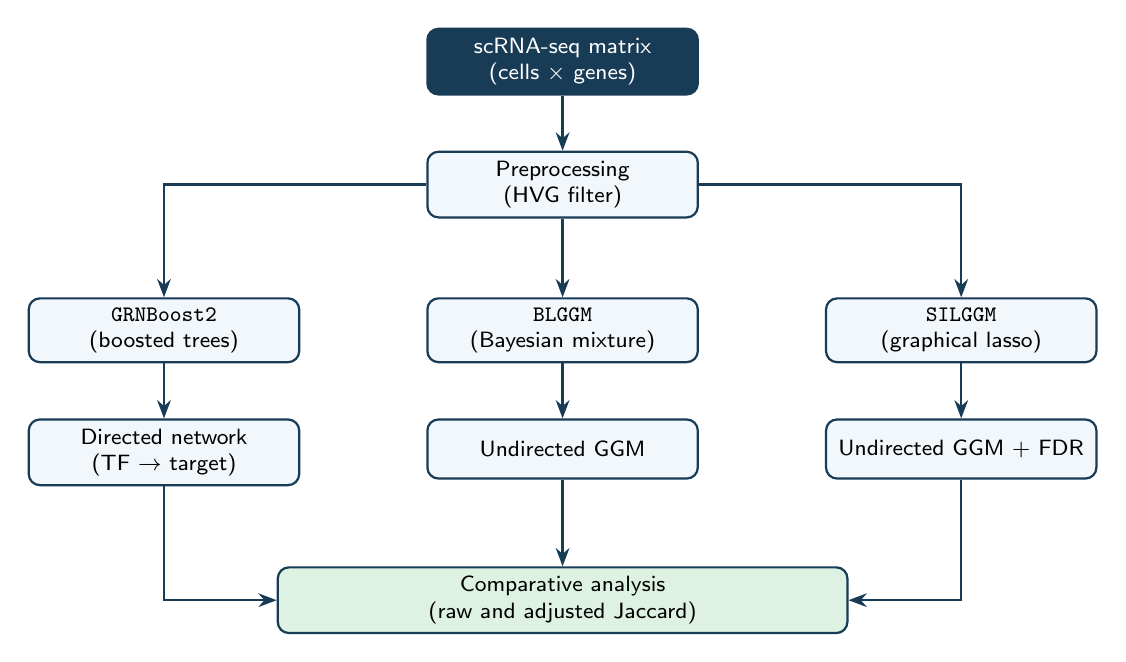
\begin{tikzpicture}[
      node distance = 0.7cm and 0.45cm,
      box/.style = {rectangle, draw=HeaderBlue, thick, fill=RowBlue,
        text width=3.2cm, align=center, rounded corners,
        minimum height=0.75cm, font=\sffamily\footnotesize},
      arrow/.style = {thick, -{Stealth}, draw=HeaderBlue}
    ]
    \node (A) [box, fill=HeaderBlue, text=white]
      {scRNA-seq matrix\\(cells $\times$ genes)};
    \node (B) [box, below=of A] {Preprocessing (HVG filter)};
    \node (C) [box, below left=1.0cm and 1.6cm of B]
      {\texttt{GRNBoost2}\\(boosted trees)};
    \node (E) [box, below=1.0cm of B]
      {\texttt{BLGGM}\\(Bayesian mixture)};
    \node (F) [box, below right=1.0cm and 1.6cm of B]
      {\texttt{SILGGM}\\(graphical lasso)};
    \node (G) [box, below=of C] {Directed network\\(TF $\rightarrow$ target)};
    \node (K) [box, below=of E] {Undirected GGM};
    \node (L) [box, below=of F] {Undirected GGM + FDR};
    \node (P) [box, fill=YesBackground, below=1.1cm of K, text width=7cm]
      {Comparative analysis\\(raw and adjusted Jaccard)};
    \draw [arrow] (A) -- (B);
    \draw [arrow] (B) -| (C);
    \draw [arrow] (B) -- (E);
    \draw [arrow] (B) -| (F);
    \draw [arrow] (C) -- (G);
    \draw [arrow] (E) -- (K);
    \draw [arrow] (F) -- (L);
    \draw [arrow] (G) |- (P);
    \draw [arrow] (K) -- (P);
    \draw [arrow] (L) |- (P);
  \end{tikzpicture}
  \caption{GRN benchmark pipeline after dropping literature-embedding
    graph networks. GRNBoost2, BLGGM and SILGGM share the same filtered
    matrix; Jaccard is computed on symmetrised edge sets.}
  \label{fig:pipeline}
\end{figure*}

\section{Results}
\label{sec3}

We score engineering feasibility, computation, and topological overlap.
Reported numbers are those of the internship on the 500-gene
gastruloid slice; they are not re-estimated in this template.

\subsection{Engineering}
Table~\ref{tab:eng} summarises installation burden. Easy means a
standard language stack; Medium means CRAN/R configuration; Hard means
compiling native code (OpenMP) or pinning GPU stacks.

\begin{table}[t]
\caption{Software characteristics (internship assessment).}
\label{tab:eng}
\begin{tabularx}{\columnwidth}{lXc}
\toprule
Method & Stack & Install \\
\midrule
GRNBoost2 & Python / Arboreto & Easy \\
SILGGM & R / CRAN & Medium \\
BLGGM & R / GitHub, OpenMP & Hard \\
\bottomrule
\end{tabularx}
\end{table}

\subsection{Computation}
On the 500-gene table, GRNBoost2 finished in about 30\,s and returned
26{,}615 directed edges. BLGGM needed about nine hours of MCMC for
3{,}029 high-confidence undirected edges. SILGGM sits between these
extremes in the frequentist GGM class; exact wall times belong in the
companion scripts once inputs are frozen.

\subsection{Overlap}
Let $A$ and $B$ be edge sets. Raw Jaccard is
\begin{equation}
J_{\mathrm{raw}}(A,B)=\frac{|A\cap B|}{|A\cup B|}.
\end{equation}
Coverage differs sharply across methods, so we also use a chance-adjusted
index
\begin{equation}
J_{\mathrm{adj}}=\frac{J_{\mathrm{raw}}-E[J_{\mathrm{raw}}]}{1-E[J_{\mathrm{raw}}]}.
\end{equation}
BLGGM and SILGGM, despite Bayesian versus frequentist implementations,
showed a stronger independent consensus on partial-correlation edges
than either did with the dense GRNBoost2 graph. That pattern is
expected if both GGMs filter confounding co-expression.

\section{Discussion}
\label{sec4}

Limitations include the lack of a gold-standard network, sensitivity to
regularisation (lasso $\lambda$, FDR $\alpha$, MCMC length, mixture
$K$), and runtime disparity. Nonparanormal shrinkage or truncation
\cite{liuNonparanormalSemiparametricEstimation2009} in
\CRANpkg{huge} \cite{R-huge} is the default Gaussian-copula pre-step for
SILGGM because raw counts are not Gaussian. BLGGM instead models dropout on
library-normalised non-negative data \cite{wuEstimatingHeterogeneousGene2022}.

Code and launch headers for \texttt{Rscript}/\texttt{nohup} are in
\url{https://github.com/bastienchassagnol/DeCovarT_reproducibility}.

\bibliography{../bibliography/REFERENCES,../bibliography/packages}
\end{document}
